\documentclass[11pt,a4paper]{article}
\usepackage[utf8]{inputenc}
\usepackage[spanish]{babel}
\usepackage{amsmath}
\usepackage{amsfonts}
\usepackage{amssymb}
\usepackage{graphicx}
\usepackage[left=2cm,right=2cm,top=2cm,bottom=2cm]{geometry}
\title{\textbf{Universidad Politécnica de la Zona Metropolitana de Guadalajara\\
Ing. Mecatrónica}}
\date{29 de septiembre del 2019}
\begin{document}

\maketitle

\begin{figure}[hbtp]
\centering

\includegraphics[scale=1]{1.jpeg}
\end{figure}




\begin{center}
\author{Alumno: Barrera Vazquez Omar}
\\{Asignatura: Sistemas de interfaz de usuario}
\end{center}


\newpage

\section{¿Que es un \emph{tiristor}?}

un tiristor es una combinación de un transistor y un diodo rectificador, ya que en su funcionamiento también requiere superar un voltaje para permitir conducir la corriente de cierto modo, pero también puede hacer la función de un transistor, esto variara según el tipo de tiristor que se maneje, es un semiconductor que se maneja en cinco presentaciones (\emph{diodo shockley, SCR,GCS,SCS,DIAC y TRIAC}).

En los siguientes apartados se podrá observar un análisis complementario sobre los \emph{tiristores} y su funcionamiento antes de pasar al siguiente tema que es \emph{\textbf {activación de circuitos con tiristores en convertidores CA-CD y CA-CA}}.
Esto tiene que tener bases fundamentales sobre el funcionamiento de los tiristores, para realmente entender como se comporta en distintos tipos de convertidores.

\section{Funcionamiento de un \emph{tiristor}}

Un tiristor se compone por cuatro capas como si fuera un transistor, esta configuración le permite trabajar como un diodo el cual conduce un voltaje y que al ser superado en cierto punto de la recta, hace una regresión de tension hasta llegar a menos de un 1\emph{volt} y en el mismo lapso de tiempo su intensidad se elevara, lo que nos indica que esta haciendo la conducción.

\begin{itemize}

\item \textbf{diodo Shockley} 
Este tipo de tiristor es el de funcionamiento básico y acoplado en cuatro capas y es de una solo conducción, su conformación es como lo muestra la siguiente imagen;


\begin{figure}[hbtp]
\centering
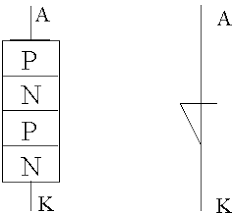
\includegraphics[scale=0.7]{3.png}
\end{figure}



\item \textbf{SCR (Silicon Controlled Rectifica)}
De igual manera en cuestión de funcionamiento que el \emph{diodo Shockley}, solo que agrega una función extra denominada \textbf{Gate} (puerta), el cual por medio de pulsaciones de tension es que lograr elevar su voltaje en diferentes etapas y se conforma de la siguiente manera;

\begin{figure}[hbtp]
\centering
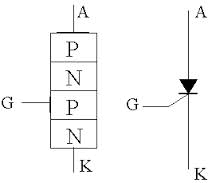
\includegraphics[scale=0.7]{2.png} 
\end{figure}

\newpage

\item \textbf{GCS (Gate Controlled Switch)}
Este tipo de tiristor trabajo igual que el \emph{SCR} solo que maneja intensidades y tensiones mas bajas, pero sus pulsos son manejados por pulso negativo 10 a 20 veces mas pequeño, se muestra de la siguiente manera:


\begin{center}
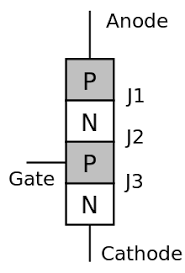
\includegraphics[scale=0.5]{4.png}
\end{center}

\item \textbf{SCS (Silicon Controlled Switch)}
La cualidad de este tiristor es que tiene dos \textbf{gate}, por lo que puede conducir de manera bidireccional lo que le proporciona mayor utilidad a comparación de sus antes mencionados, su símbolo es el siguiente;


\begin{figure}[hbtp]
\centering
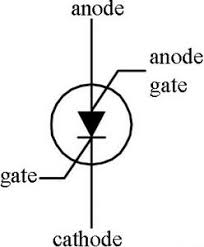
\includegraphics[scale=0.5]{5.jpeg} 
\end{figure}


\item \textbf{DIAC}
Es básicamente el mismo funcionamiento que un tiristor normal solo que este conduce de manera direccional por lo que se hace multipropiedad, su símbolo se en la siguiente imagen;

\begin{figure}[hbtp]
\centering
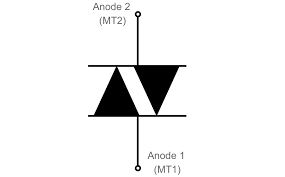
\includegraphics[scale=0.5]{6.png} 
\end{figure}

\item \textbf{TRIAC}
Con la misma función que el \emph{DIAC}, trabaja de la misma manera solo que se agrega una \textbf{gate} que ayuda a multiplicar sus funciones y su símbolo solo es agregado el símbolo de gate, como se muestra en la figura;

\begin{figure}[hbtp]
\centering
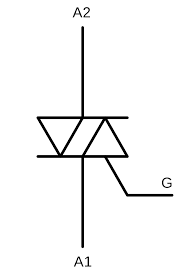
\includegraphics[scale=0.5]{7.png} 
\end{figure}

\end{itemize}

\section{\emph{Tiristores en convertidores CA-CD}}
La utilización de los tiristores en la electrónica de potencia tiene múltiples beneficios a comparación de los diodos rectificadores, estos tienen mayor rango de operación y ademas permite controlar el disparo de activación de este. Por lo que se puede controlar el angulo de salida de la corriente.

Para hacer que funcione como un convertidor de CA-CD es necesario poner dos tiristores SCR en modo anti paralelo, esto para que no deje transmitir tension. Una de sus ventajas como rectificador es que el rizado que produce es muy despreciable lo que lo hace mejor rectificador. 

el posicionamiento en un circuito convertidor, es el mismo que el de los diodos rectificadores, solo es cuestión de asegurarse en la posición con la que se alimentara el SCR, lo podemos observar en la siguiente imagen;

\begin{figure}[hbtp]
\centering
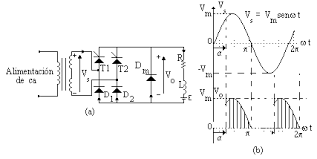
\includegraphics[scale=1]{8.png} 
\end{figure}

En la imagen \textbf{(a)} se puede observar la conformación de un circuito convertidor donde son aplicados dos \emph{SCR} de manera paralela, de esta manera harán la conducción hacia un solo sentido del circuito. Mientras tanto en la figura \emph{(b)} podemos encontrar la salida del circuito convertidor.

\section{\emph{Tiristores en convertidores CA-CA}}
Los convertidores de \emph{CA-CA} son utilizados de manera que se cambia alguna o algunas de las características de la onda senoidal. Puede ser propiedades como \textbf{frecuencia, tension y ciclos}, por lo que hay distintos tipos de convertidores. Para estudiar el uso de los tiristores en los convertidores, comenzaremos con el mas básico, que es el \emph{modificador de tension}, por lo que da una tension diferente con una frecuencia fija. observemos la siguiente imagen;

\begin{figure}[hbtp]
\centering
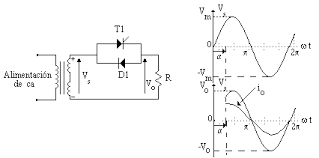
\includegraphics[scale=1]{9.png}
\end{figure}

\newpage

\section{Reseña}
Los tiristores tienen muchas cualidades extras que los diodos rectificadores no manejan, por lo que a su costo-beneficio es mejore utilizarlos en lo convertidores de tension, mejora ciertos aspectos como; disminución del rizado, control sobre cuando ejecutar la conversión, algunos son bidireccionales por lo que conducen de dos maneras y para terminar son de manejo en alta potencia.




\end{document}